\section{La professione del medico di medicina generale raccontata}

\subsection{Introduzione}

La medicina generale è una disciplina (apprendimento nel tempo) con
contenuti clinici, educativi e di ricerca orientata alle cure primarie.
Il medico di medicina generale collabora e si coordina con i colleghi
del territorio, dell'ospedale e gli universitari. L'attività del medico
di base è incentrata sulla famiglia, sull'individuo e sulla persona. Il
suo compito è quello di erogare le \textbf{cure primarie}, che sono cure
in primo luogo di \emph{attese opportunità} (l'utente si rivolge
direttamente al suo medico al momento del bisogno, cure in acuto) e di
libero accesso a tutti i cittadini. In secondo luogo vengono erogate
cure continue (croniche) e qui parliamo di \emph{medicina di
iniziativa}. Le cure croniche richiedono che il medico segua il paziente
più intensamente, contattandolo anche telefonicamente o concordando con
anticipo controlli e interventi. Il medico di base si occupa di tutte le
problematiche della persona passando dall'unghia incarnita allo
scompenso cardiaco. Un altro punto importante è quello di essere
inseriti nella \emph{comunità di riferimento}: secondo le normative il
medico di base può arrivare a 1500 assistiti che lo scelgono. È
necessario mantenersi informati sulla prevalenza delle malattie della
propria comunità. Il medico diventa parte integrante della sua comunità
e quindi è importante farsi stimare e diventare un punto di riferimento
con responsabilità specifiche. Non viene più seguito il paradigma
paternalistico medico-paziente ma il \emph{paradigma
bio-medico-psicosociale} e il \emph{modello olistico} (la persona nel
suo insieme e non a singoli apparati); un essere vivente rimane per
molti aspetti misterioso. Bisogna saper fare (applicare il sapere alla
pratica) ma soprattutto saper essere, saper gestire le risorse, saper
comunicare ed è necessaria la capacità di saper contestualizzare e
personalizzare. Una delle attività fondamentali è quella della
\textbf{prevenzione della salute} che non significa solo consigliare di
non fumare, non bere e fare attività fisica ma anche stimolare il
benessere psicofisico in sé.

\subsection{L'importanza della collaborazione}

Adesso visualizzeremo un filmato che ci farà capire l'importanza della
collaborazione che diventa fondamentale per far fronte a quella che è
l'\textbf{epidemia della cronicità} (patologie croniche e difficoltà del
vivere, il malessere delle persone è in aumento soprattutto tra i
giovani con manifestazioni patologiche psicosomatiche).
\\\\
Di seguito gli interventi di ogni specialista.
\\\\
MMG: la signora si è un po' aggravata ultimamente, sono peggiorate le
sue condizioni tanto che nel breve periodo è prevedibile un exitus. Come
sapete c'erano tanti pareri specialistici riguardo alla PEG però poi per
alcuni motivi non si è riuscito a impiantarla. Il collega chirurgo ci ha
aiutato moltissimo perché è riuscito ad inserire, nonostante la stenosi
dell'esofago, il catetere e quindi siamo riusciti ad andare avanti con
le terapie. Qualche giorno fa la signora, con un gesto improvviso, si è
tolta il catetere e si è provato con l'aiuto dell'infermiera a
riposizionarlo. L'operazione sembra riuscita e adesso pare sia tutto a
posto ma si richiede il parere dello specialista ospedaliero per quanto
riguarda il corretto posizionamento.
\\\\
CHIRURGO: noi dell'Azienda Ospedaliera abbiamo a disposizione uno spazio
temporale per questo progetto che è al cambio del turno, quindi per ora
di pranzo. Per quest'ora c'è la possibilità di recarsi al domicilio
della signora per controllare il posizionamento del sondino
naso-gastrico e inserire i dati nella cartella informatizzata per
mettere tutti al corrente della situazione.
\\\\
INFERMIERA: come avevo già detto al medico curante noi non riusciamo più
a trovare delle vene quindi per noi diventa quasi impossibile proseguire
la terapia parenterale concordata. Tanto è vero che ieri abbiamo
iniziato provvisoriamente un'ipodermoclisi per somministrare liquidi
{[}\emph{La ipodermoclisi è una tecnica che consiste nella
somministrazione sottocutanea di grandi quantità di liquidi ed
elettroliti (soluzione salina allo 0.8\% o allo 0.45\%), al fine di
ricostituire il patrimonio idrosalino di pazienti modicamente
disidratati, in cui sia impossibile la somministrazione per via orale od
endovenosa. È utile anche per la somministrazione di glucosio al 5\%.
Essa risulta particolarmente indicata in pazienti con problemi di
deglutizione o con vene molto sottili e particolarmente fragili. La
somministrazione va effettuata con un comune ago butterfly,
preferenzialmente in sede addominale, ascellare o toracica
sottoclavicolare (con possibilità di rotazione delle sedi),
eventualmente aggiungendo l'enzima ialuronidasi che facilita la
diffusione{]}.} Era stato richiesto il posizionamento di un catetere
venoso centrale quando la signora era ancora ricoverata in ospedale ma
per qualche disguido è stata dimessa senza che le venisse posizionato.
Con il sondino si riesce abbastanza a proseguire le terapie sia
farmacologiche che idratanti però sicuramente noi ci sentiremmo più
tranquille se qualcuno venisse a controllare il sondino onde evitare
lesioni o rigurgiti in sede del tumore.
\\\\
CHIRURGO: io direi che domani possibilmente insieme, se riusciamo a
coordinarci in questo intervallo, possiamo passare a casa della paziente
e vedere di riuscire ad incannulare una vena centrale, già problematica
al momento del ricovero per le sue condizioni . Comunque bisogna
risistemare il sondino naso gastrico, proseguire con la terapia
idratante attraverso il sondino e ipodermoclisi perché il problema
dell'incannulamento era stato già importante durante il ricovero.
\\\\
ASSISTENTE SOCIALE: come servizio sociale abbiamo attivato l'igiene
personale per la signora due volte al giorno e un pasto una volta al
giorno, confezionato sia per lei che per il marito. La situazione
familiare rimane però un po' problematica e delicata. In casa c'è il
figlio e sappiamo che è in cura al SerT e il marito non è consapevole
fino in fondo della gravità della situazione della moglie. Per cui
quando arriviamo magari le stanze sono fredde e poi non riesce a fare
lui l'altro pasto della giornata. Quindi finchè il figlio sta bene ed è
compensato la situazione va abbastanza bene.
\\\\
MEDICO SERT: il figlio al momento appare in un discreto compenso, è
compliante alla terapia, sta seguendo anche una psicoterapia per la
prima volta, probabilmente ha preso consapevolezza della situazione
della madre. Io sono stata chiamata qui per capire se la signora può
continuare a seguire un'assistenza domiciliare perché ultimamente il
figlio aveva avuto degli atteggiamenti aggressivi e poco adeguati. Mi
sono consultata anche con i colleghi psicologi e in realtà adesso è in
un momento molto tranquillo per cui io direi che si può continuare ad
accedere al domicilio e se ci fossero dei problemi anche noi del SerT
siamo a disposizione.
\\\\
INFERMIERA: senz'altro la famiglia è molto problematica e comunque ci
assorbe un sacco di energie e risorse territoriali. Noi andiamo un po'
in sofferenza onestamente il sabato e la domenica perché c'è solo
un'infermiera in turno per tutta la città per cui diventa un po'
difficile. Diciamo che il lavoro in gruppo ci aiuta un attimino a
condividere e a dividerci le responsabilità e senz'altro il medico di
continuità assistenziale ci da una mano, ci consiglia ed è sempre
presente. Una proposta che vorrei condividere col gruppo sarebbe di
coinvolgere il volontariato, soprattutto per sostenerci durante i giorni
critici o le festività.
\\\\
MMG: questa è un' ottima idea che dovremmo approfondire con l'azienda
per trovare il modo di integrare le due cose. In effetti se non ci fosse
l'aiuto dei servizi infermieristici territoriali questo sarebbe un
classico caso da ricovero in strutture intermedie o in letti
osservazionali della Casa della Salute ma non sono sicuro che la
famiglia avrebbe accettato questo tipo di intervento.
\\\\
CARDIOLOGO: io ho sentito direttamente lui stamattina con il cellulare e
mi ha descritto il problema sopraggiunto dell'aritmia e
dell'ipotensione, ma in accordo con lui non aggiungerei altri farmaci
alla terapia già in atto perché la sintomatologia cardiaca è
verosimilmente legata allo squilibrio elettrolitico dovuto alla malattia
a questo stadio. Pertanto a mio parere se l'aritmia è ben tollerata non
deve essere trattata; qualunque eventuale trattamento deve essere
incentrato solamente sul controllo dei sintomi.
\\\\
GUARDIA MEDICA: anche io non ho notizie nuove. I colleghi mi tengono
informato e le cose sono stazionarie. Devo congratularmi però con il
medico di medicina generale perché da tempo vedo che il dolore è
perfettamente controllato con i cerotti transdermici e non sono stati
evidenziati assolutamente effetti collaterali. Le chiamate alla
continuità assistenziale sono state rare fino ad ora, ma siamo comunque
pronti e informati grazie a queste riunioni di team e al sistema
informatizzato.
\\\\
MMG: la nostra collaborazione con i colleghi infermieri credo che
funzioni molto bene. I compiti per questa settimana sono stati divisi,
bisogna solo tenersi informati tramite la cartella informatizzata. Una
cosa importante per l'infermiera: domenica sono in città e l'accesso lo
farò io.
\\\\
Verbale finale: il collega chirurgo passerà a riposizionare il sondino,
poi si proseguirà con l'idratazione tramite sondino e ipodermoclisi. La
prossima riunione sarà a fine mese.

\subsection{Caso clinico}

Noi medici di medicina generale dobbiamo guardare la persona nel suo
insieme, considerando anche che spesso la compliance del paziente non
rientra nelle linee guida canoniche.
\\\\
Questo paziente in particolare si è presentato 4 volte in ambulatorio
negli ultimi 4 mesi e in più ci sono stati anche contatti telefonici
(circa 5) e e-mail. Quindi è un paziente che si è visto spesso. È un
paziente maschio di 50 aa, con un figlio piccolo, pratica sport, è molto
attivo e viaggia spesso. Segue molto attentamente l'attualità,
considerando anche che il suo è un lavoro molto tecnico all'interno di
un giornale. Non fuma, ha uno stile di vita sano e in terapia ha solo un
PPI e assume occasionalmente antiinfiammatori per il mal di schiena. È
molto pignolo e attento ad assumere prodotti naturali. Dal 1980 questo
paziente lamenta mal di pancia, scariche diarroiche in particolare nei
periodi di stress. I sintomi riportati non sono precisi (ad esempio
dolore epigastrico) ma vaghi e mal localizzati. Si è giunti a fare esami
diagnostici (rx, gastroscopie, colonscopie ecc.. ) e visite
gastroenterologiche perchè come sempre il paziente è un mistero e non si
può in nessun caso sottovalutare la sintomatologia e non prendere in
considerazione ogni eventualità. Il risultato di queste visite ed esami
era nella norma con niente da segnalare. I sintomi si alleviavano per un
periodo poi ritornavano e alla fine dopo mille consulenze ci si orienta
verso una Sindrome da Colon Irritabile. Dopo un decennio la
sintomatologia cambia, sempre sintomi aspecifici, però ci si sposta dal
settore gastroenterico al comparto muscolare. Si prova ad iniziare una
terapia con FANS ma non si otterrà nessun beneficio riferito. Seguono
successivi esami ematici il cui risultato sarà nella norma, esami
strumentali anch'essi nella norma e visite specialistiche che non
segnaleranno nessun quadro patologico. Lamentava anche insensibilità al
pavimento pelvico e per questo si è sospettata una sindrome da cauda
equina, smentita poi dagli esami eseguiti. Nel 1996 l'anamnesi riporta
l'asportazione di una cisti tendinea nell'avambraccio. Passa un altro
decennio e ricompaiono i sintomi iniziali, quindi mal di pancia ed
episodi diarroici che il paziente cerca di giustificare riportando
informazioni apprese da internet. Vengono nuovamente eseguiti esami
specialistici da cui nuovamente non emerge nulla. La sintomatologia
sembra alleviarsi o addirittura sparire per un certo periodo di tempo
(il 20-30\% degli accessi dal medico di base sono per patologie
psicosomatiche e funzionali, se si dovessero fare esami strumentali e
visite specialistiche per ognuno il sistema sanitario nazionale
crollerebbe). La diagnosi rimane indirizzata sulla IBS, quindi una
patologia funzionale. Poi fa una risonanza privatamente e riscontra un
angioma ma questo, visto le ridotte dimensioni, non poteva comunque
giustificare la sintomatologia. Nonostante questo, nel 2016 decide per
suo conto di ripetere un'altra risonanza che darà lo stesso identico
referto, quindi sospetto angioma. Il radiologo non poteva visualizzare
la risonanza precedente e quindi richiede una TAC di conferma. Il
paziente esegue la TAC che conferma l' angioma di piccole dimensioni e
di nessuna importanza clinica. Allo stato attuale continua a chiamare
per richiedere visite fuori dagli orari, cerca di non rispettare i turni
della sala d'aspetto e in ogni incontro i sintomi vengono sempre
ripresentati e cerca di far credere che non sia mai stato affrontato il
problema. È un caso estremamente semplice guardando la diagnosi finale,
non ci sono patologie mediche alla base degne di nota o comunque
particolarissime. Questo è un paziente tipico nella medicina generale,
solo a un livello un po' esasperato per quanto riguarda ansia e
richieste. Voi non sceglierete i pazienti ma saranno loro a scegliere
voi. È più difficile lavorare come medici di base che come medici di
guardia medica.
\\\\
È importante che qualunque concetto abbiate del paziente (rompiscatole,
psicosomatico, funzionale ecc..) non influenzi l'obiettività sulla
sintomatologia riportata. Gli errori possono sempre accadere ma bisogna
saperli affrontare.
\\\\
Breve storia: un chirurgo aveva consultato un medico legale perchè aveva
sbagliato completamente un intervento e la paziente si trovava in
terapia intensiva. Il medico legale non sapeva cosa consigliare al
chirurgo e l'unica cosa che gli ha raccomandato era di stare accanto
alla paziente più che poteva per farle capire che per qualsiasi
conseguenza dovuta all'intervento lui sarebbe stato disponibile. Il
chirurgo dal giorno successivo si è messo accanto alla paziente ed è
rimasto lì vicino anche ai familiari. Poi purtroppo la donna è deceduta
ma lui è stato ringraziato per la dedizione; i parenti non avevano
sospettato che il chirurgo avesse sbagliato l'intervento poiché il
decesso era comunque tra le complicanze. Però la dedizione e la
vicinanza che il chirurgo ha avuto nei confronti di questa signora ha
portato i parenti a ringraziarlo.

\subsection{Attività del medico di medicina generale}

Una grande caratteristica della medicina generale è la \textbf{fiducia}
e la vicinanza con il paziente. Guardando a numeri e statistiche i
medici di medicina generale sono la classe medica con meno denunce
rispetto alle altre classi.

La soluzione è diventare psicologi di se stessi, competenti nella
comunicazione e non essere mai presuntuosi perché se no si entra in
conflitto anche per cose di piccolo conto a cui segue la denuncia.

\begin{figure}[!ht]
\centering
	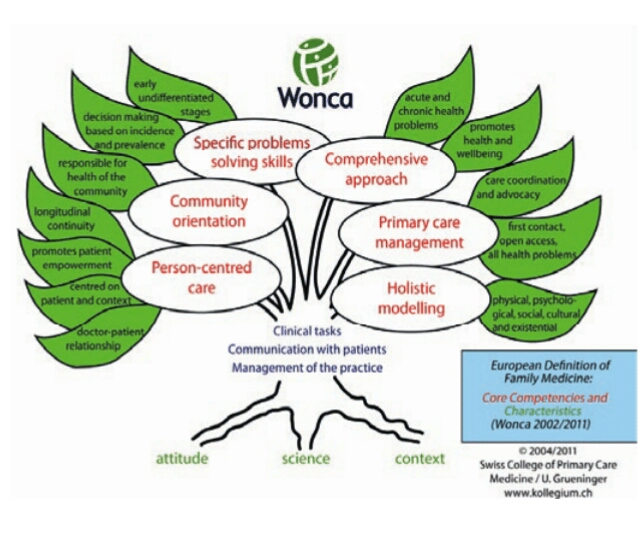
\includegraphics[width=0.8\textwidth]{39/image1.jpeg}
	\end{figure}
	
Ci sono anche altre cose che il medico di base fa sul territorio come ad
esempio l'\textbf{associazionismo}. L'attività sul territorio è
importante soprattutto per quanto riguarda l'aspetto della cronicità che
è enorme: siamo ancora molto lontani dall'affrontarlo con adeguatezza
perché siamo ancora molto indietro nei percorsi diagnostici terapeutici
assistenziali (PDTA) che dovrebbero coinvolgere tutti (servizi,
territorio, ospedale e università). Io spesso aggiungo la lettera R
(PDTA-R) poiché per me è importante la \textbf{relazione} tra colleghi e
all'interno di un team, cioè quello che avete visto prima nel filmato
che vi ho proiettato. I team possono essere multiprofessionali (medici,
infermieri) ma anche multidisciplinari (che coinvolgono figure come
quella dell'assistente sociale).
\\\\
Molto importante è l'\textbf{assistenza domiciliare} che cambia in base
al tipo di visita richiesta poiché quella di un malato terminale
richiede tempo e pazienza. È molto complicato e impegnativo fare bene
questo mestiere. Se insorgono dei problemi o delle mancanze va a rotoli
tutto perché salta il pronto soccorso, salta l'ospedale, saltano i
ricoveri.
\\\\
È anche importante la \textbf{medicina di iniziativa} perché si
richiamano i pazienti prima che smettano di avere una compliance fatta
bene quindi prima che inizino ad avere dei problemi.
\\\\
C'è inoltre il \textbf{servizio h12/h24} (mmg + medico continuità
assistenziale + 118). Il servizio territoriale è completo. L'h12 spetta
ai medici di base poiché essi sono in servizio attivo (non reperibili ma
disponibili ) dalle 8.00 alle 20.00. L'h12 non è assolutamente facile
perché bisogna dare questo servizio per tutte le 12h e ciò oggi si
realizza nelle medicine di gruppo e nelle case della salute.
\\\\
Poi ci sono ruoli relativi ad \textbf{attività istituzionali}. Il medico
di base non fa solo il medico ma gestisce anche delle risorse. Il
problema della gestione delle risorse, nel bene e nel male, coinvolge il
medico anche nelle istituzioni, cioè all'interno dell'organizzazione
dell'Azienda Usl, all'interno dell'organizzazione dei quartieri,
all'interno delle questioni sindacali e all'interno dell'Ordine dei
Medici.
\\\\
Poi si è adibiti alla \textbf{valutazione di primo livello vocazionale}.
Io sono anestesista, psicologo e ho fatto anche lo psichiatra quindi
metto a disposizione del gruppo le mie capacità e competenze ed è quello
che fanno tutti i componenti del gruppo. Si fa come in Francia dove i
medici che lavorano in gruppo si scrivono una lettera che inizia con
``Caro fratello'' e prosegue con ``ho visto questo paziente che
ha\ldots{}''; non è un referto specialistico, ma è già una cosa che si
può fare di primo livello che può scaricare moltissimo le liste
d'attesa.
\\\\
Altra cosa è la \textbf{docenza} sia per la scuola specifica in Medicina
Generale che per l'Università.
\\\\
Poi abbiamo la \textbf{formazione} che in genere è autoformazione; è
molto importante confrontarsi con i colleghi.
\\\\
Un'ulteriore cosa fondamentale è \textbf{essere dentro la società
civile} e quindi tutto ciò che riguarda le relazioni con il
volontariato.
\\\\
Poi si fa \textbf{ricerca} sia di tipo clinico (più complicata per noi)
ma anche secondo il paradigma bio-psico-sociale. Anni fa abbiamo
distribuito questionari riguardanti il gradimento della popolazione nei
confronti delle associazioni dei medici di base pubblicato sul Sole 24h
e un altro questionario riguardante il pensiero delle persone nei
confronti della privacy. La ricerca in medicina generale è anche di tipo
territoriale come può essere un piccolo progetto sull'utilizzo di device
(delle specie di spirometri) che si collegano con delle applicazioni al
cellulare per monitorare tutti i pazienti con BPCO, asmatici e fumatori
e vedere la compliance ma soprattutto valutare le patologie polmonari
prima che siano ad uno stato avanzato. Questo è utile per salvare quella
quota di fumatori convinti di avere i polmoni sani ma che in realtà
stanno sviluppando patologie irreversibili. Adesso il medico di base
utilizza anche delle piattaforme su cui vengono inserite le cartelle
cliniche dei pazienti e quindi tutti i dati vengono informatizzati. C'è
la Società Italiana Scientifica di Medicina Generale che ha una quota di
medici di base ritenuti di alto livello con i quali collabora per fare
delle ricerche che vengono pubblicate ed hanno già dimostrato che i loro
dati clinici, per esempio sul settore cardiologico, sono comparabili a
dati clinici di ospedali grossi. Hanno un pool di pazienti reali e
questa è una differenza tra la ricerca in medicina territoriale e la
ricerca ospedaliera perché nella ricerca ospedaliera il paziente arriva
già ``screenato'' (si sa già di cosa soffre e quale è la diagnosi)
mentre nel territorio c'è tutta un'integrazione quindi la ricerca che
emerge dal territorio ha una popolazione reale. Per esempio se emergono
5 farmaci per lo scompenso cardiaco e la Società Italiana di Medicina
Generale decide di fare una ricerca per vedere quale di questi farmaci
su questi pazienti funziona meglio, viene fuori quello che funziona più
correttamente nella popolazione reale, poi da li si traggono conclusioni
e conseguenze. Sono anche ricerche solitamente abbastanza pulite. Quindi
non dimenticare che nella medicina generale c'è ricerca e integrazione e
si possono fare tante cose importanti. A proposito di ricerca venerdì
prossimo sarò alla Bocconi a Milano perché stiamo cercando di
organizzare una ricerca sul concetto di fragilità. Proviamo insieme ai
colleghi a vedere quali sono le caratteristiche della fragilità. Una
delle fragilità più grosse che è emersa è quella dei professionisti.
All'interno della fragilità dei pazienti incide la fragilità dei
professionisti e ciò ha conseguenze sulla salute, sul suo mantenimento e
sulla prevenzione.
\\\\
La qualità diffusa e omogenea è sempre stata garantita negli ultimi anni
in tutto il Paese ed è uno dei motivi che porta il gradimento dei medici
di base a livelli molto alti.
\\\\
Art. 32 della Costituzione che viene sempre citato\emph{: ``La
Repubblica tutela la salute come fondamentale diritto dell'individuo e
interesse della collettività, e garantisce cure gratuite agli
indigenti.} \emph{Nessuno può essere
obbligato a un determinato trattamento sanitario se non per disposizione
di legge. La legge non può in nessun caso violare i limiti imposti dal
rispetto della persona umana.''}
\\\\
Garantisce cure gratuite \emph{agli indigenti} quindi sta cambiando
anche questo aspetto. È vero che ci sono i ticket e le partecipazioni ma
molte persone si sono abituate ad avere tutto e subito. Molti pazienti
richiedono la routine di esami annuali anche se è stato dimostrato che
questo non serve così tanto (es: emocromo a tappeto tutti gli anni non
serve a garantire un miglioramento nelle cure). Molti pazienti si
presentano in ambulatorio e prima ancora di illustrare la patologia per
cui si sono recati dicono di essere esenti ticket quindi alla fine
risulta difficile convincere persone abituate a fare esami di routine
tutti gli anni che questi non servono. Il medico di base ha il compito
di mettere al corrente il paziente dell'inutilità di sottoporsi ad
alcuni esami se non vi è una evidente necessità e il paziente è libero
di poter cambiare il proprio medico se questo non è di suo gradimento.
Il nostro sistema è pubblico, finanziato e strutturato in questo modo
quindi ci sono le aziende sanitarie e le aziende
ospedaliere-universitarie. Il medico è l'ufficiale sanitario di primo
livello.
\\\\
Sul piatto della bilancia abbiamo la sostenibilità del servizio,
l'innovazione delle cure primarie, la modifica del paradigma e i nuovi
modelli organizzativi. Le nostre cure primarie sono state le migliori al
mondo. Si riuscirà a mantenere questo livello? Com'è il medico di base
in Europa? Noi in Italia siamo liberi professionisti convenzionati con
il SSN. In alcuni documenti siamo definiti parasubordinati perché siamo
costretti a regole nazionali, regionali e locali, però nelle ultime
bozze dell'accordo collettivo nazionale si parla di libero
professionismo. Anche in GB e Spagna è così (in Spagna solo nella
provincia della Catalogna). In Germania, Olanda e Francia il medico è
invece convenzionato con le mutue sia pubbliche che private. In Francia
il paziente viene visitato, paga il medico e poi si fa rimborsare una \%
dalla sua mutua o dalla mutua dello Stato. Nel resto della Spagna, in
Portogallo e in Scandinavia i medici di base sono dipendenti. A Malta e
in Grecia sono un po' dipendenti e un po' convenzionati.
\\\\
Nell'area territoriale bisogna pensare ai percorsi e alle cure
intermedie proprio per ridurre l'afflusso e l'attività ospedaliera che
dovrebbe essere riservata alle acuzie.
\\\\
Come si diventa MMG oggi? Io sono diventato medico di base perché ho
scelto di farlo però oggi per diventare medico di base bisogna fare la
specialità. L'accesso alle graduatorie regionali avviene solo attraverso
l'acquisizione del diploma di specialità. Come è fatto il corso? È un
piano di studi della durata di 3 anni con un precedente test di
ingresso. È costruito su \emph{attività seminariali} suddivise in
\emph{seminari interdisciplinari} e \emph{seminari clinici}. Quelli
interdisciplinari sono un po' più vicini all'attività della medicina
generale (come si fa la ricetta medica, problem solving..) mentre i
clinici sono quelli che fate voi, più approfonditi e specialistici
(febbre, edema, prurito, patologie cardiovascolari..)
\\\\
Poi ci sono le attività pratiche che sono i \emph{tirocini}:

\begin{itemize}
\item[1.]
  tirocini ospedalieri (solo osservazionali)
\item[2.]
  tirocini nei servizi territoriali (sempre osservazionali, es. al Sert)
\item[3.]
  tirocini dal mmg che sono operativi.
\end{itemize}

Il mmg ogni giorno affronta molti problemi e non vere patologie e
malattie, si trova davanti a paradossi. L'assistenza domiciliare è molto
importante.

I clienti interni sono i professionisti che lavorano all'interno del SSN
mentre i clienti esterni sono i pazienti. I bisogni di entrambi sono
eterogenei e non standardizzabili. La scientificità dei medici è la
capacità di riuscire a personalizzare la cura per ogni persona.

\subsubsection{Favola per capire gli effetti dei preconcetti}

C'era una volta un cammelliere che aveva 3 figli e sentendosi prossimo
alla sua dipartita decide di fare testamento. Sceglie di lasciare i suoi
beni ai figli però divide il patrimonio in modo tale che metà spettasse
ad un figlio, 1/4 ad un altro figlio e 1/6 spettasse all'ultimo. Dopo la
sua morte i figli aprono il testamento e scoprono che la linea
testamentaria patrimoniale è composta da 11 cammelli. Quindi metà (5,5
cammelli) al primo figlio, 1/4 (2,75 cammelli) al secondo e 1/6 (1,8
cammelli ) al terzo. A questo punto i fratelli entrano in conflitto,
iniziano a litigare e si offendono e stanno per uccidersi. Nel frattempo
passa un altro cammelliere e si fa raccontare la storia del testamento
poi pensa a cosa si potrebbe fare e trova una soluzione. Prende un
cammello e lo va ad unire agli altri 11 cammelli, così il totale ora è
12. Quindi metà sono 6, 1/4 sono 3 e 1/6 sono 2. Cosi mette a posto i 3
fratelli. Poi riprende il suo cammello e se ne va.